\documentclass[a4paper, 12pt]{article}

\usepackage[T2A]{fontenc}
\usepackage[utf8]{inputenc}
\usepackage[english, russian]{babel}
\usepackage[left=19mm,right=19mm,top=2cm,bottom=2cm,bindingoffset=0cm]{geometry}
\usepackage{amsmath, amsfonts, amssymb, amsthm, mathtools}
\usepackage{enumitem}
\usepackage{setspace}
\usepackage{amsmath}
\usepackage{caption}
\usepackage{graphicx}
\graphicspath{{img/}}
\DeclareGraphicsExtensions{.png,.jpg}

\begin{document}
\begin{spacing}{1.5}
\setlength{\parindent}{0ex}

\section*{Семинар 4}


\subsection*{Собственные векторы и собственные значения}

\textbf{Определение 4.1.} 
Пусть $L $ - линейное пространство, $A: L \rightarrow L$ - линейное преобразование. \textit{Собственным вектором} линейного преобразования $A$ называется такой ненулевой вектор $x\in L$, что для некоторого $\lambda \in \mathbb{R}$ верно: $Ax = \lambda x$.

\textbf{Определение 4.2.} \textit{Собственным значением} линейного преобразования $A$ называется такое число $\lambda$, для которого существует собственный вектор, т.е. уравнение $Ax= \lambda x$ имеет ненулевое решение.

\textbf{Упражнение 4.1.} Найти собственные значения и собственные векторы линейных операторов, заданных в некотором базисе матрцами:
\begin{align*}
a) 
\begin{pmatrix}
-1 & 3 & -1 \\
-3 & 5 & -1 \\
-3 & 3 & 1
\end{pmatrix}; \hspace{12mm}
b) 
\begin{pmatrix}
0 & 1 & 0 \\
-4 & 4 & 0 \\
-2 & 1 & 2
\end{pmatrix}.
\end{align*}

\underline{Решение}:

\setlength{\leftskip}{5ex}
\setlength{\rightskip}{5ex}

\textbf{a)} Ищем такие $\lambda$, что у системы $Ax = \lambda x$ существует ненулевое решение:
$$Ax= \lambda x \Leftrightarrow Ax = \lambda Ex \Leftrightarrow Ax - \lambda Ex = 0 \Leftrightarrow (A - \lambda E)x = 0$$

Матричное уравнение будет иметь вид:
\begin{align*}
\begin{pmatrix}
    -1 - \lambda & 3 & -1 \\
    -3 & 5 - \lambda & -1 \\
    -3 & 3 & 1 - \lambda
\end{pmatrix}
\begin{pmatrix}
    x_1 \\
    x_2 \\
    x_3
\end{pmatrix}
=
\begin{pmatrix}
    0 \\
    0 \\
    0
\end{pmatrix}
\end{align*}

Поскольку мы хотим, чтобы однородная система обладала нетривиальным решением (в силу того что собственный вектор не может быть нулевым), матрица системы обязана быть вырожденной, т.е. иметь линейно зависимые строки или столбцы. В нашем случае собственными значениями будут $\lambda_1 = 1$, $\lambda_2 = \lambda_3 = 2$ (на занятии, когда мы познакомимся с определителем матрицы и характеристическим многочленом, станет понятно, почему $\lambda = 2$ встречается дважды).

Теперь подставим $\lambda_i$ в систему и найдём собственные векторы. Я опущу выкладки и напишу сразу (а вы проверьте!), что векторы вида $x = c_1 (1, 0, -3)^T + c_2 (0, 1, 3)^T$, где $c_1$ и $c_2$ не равны одновременно нулю, являются собственными для $\lambda = 2$, а векторы вида $x = c_3 (1, 1, 1)^T$ являются собственными для $\lambda = 1$.

\textbf{b)} Сделайте сами :)

\setlength{\leftskip}{0ex}
\setlength{\rightskip}{0ex}


\subsection*{Инвариантные подпространства}

\textbf{Определение 4.3.} Подпространство $W$ линейного пространства $V$ назвается \textit{инвариантным относительно линейного преобразования} $\varphi: V \rightarrow V$, если $\varphi(W) \subset W$.

\textbf{Определение 4.4.} \textit{Собственным подпространством} линейного преобразования $A$, отвечающим собственному значению $\lambda$, называется множество всех собственных векторов $x \in L$, соответствующих $\lambda$, дополненное нулевым вектором: $E_{\lambda} = \{ x \in L | \ Ax = \lambda x\}$.

\textbf{Упражнение 4.2.} Доказать, что ядро, образ и собственное подпространнство линейного оператора $\varphi$ инвариантны относительно $\varphi$.

\underline{Решение}:

\setlength{\leftskip}{5ex}
\setlength{\rightskip}{5ex}

\textbf{1.} Пусть $x \in \text{Ker } \varphi \Rightarrow \varphi (x) = 0 \in \text{Ker } \varphi$ (ноль, очевидно, лежит в ядре).

\textbf{2.} Пусть $x \in \text{Im } \varphi \Rightarrow \varphi (x) = y \in \text{Im } \varphi$ (по определению образа).

\textbf{3.} Пусть $x \in E_{\lambda} (\varphi) \Rightarrow \lambda x \in E_{\lambda} (\varphi)$. С другой стороны $\varphi(x) = \lambda x \Rightarrow \varphi (x) \in E_{\lambda} (\varphi)$.

 
\setlength{\leftskip}{0ex}
\setlength{\rightskip}{0ex}


\subsection*{Вырожденные преобразования}

\textbf{Определение 4.5.} Матрица, определитель которой равен нулю, называется \textit{вырожденной} (понятие определителя появится позже). Эквивалентные условия вырожденности:
\begin{itemize} [noitemsep] 
    \item Строки или столбцы матрицы линейно зависимы.
    \item $A$ - вырождена $\Leftrightarrow$ существует ненулевой вектор $x: Ax = 0$.
    \item $A$ - вырождена $\Leftrightarrow$ $\lambda = 0$ является собственным значением.
\end{itemize}
На самом деле правая часть второго пункта также означает, что ядро нашего преобразования нетривиально, т.е. содержит не только нулевой вектор. Вообще говоря, верно

\textbf{Утверждение.} Ядро тривиально, тогда и только тогда, когда отображение \textit{инъективно}, т.е. разные элементы переходят в разные. 

\textbf{Доказательство.} Ker $\varphi = \{0\} \Rightarrow \varphi$ - инъективно. Предположим противное. Пусть $\exists x \neq y: \varphi(x) = \varphi(y) \Rightarrow \varphi(x-y) = 0 \Rightarrow x-y \in \text{Ker } \varphi$ - противоречие, т.к. $\text{Ker } \varphi = \{ 0\}$, но $x - y \neq 0$.

В другую сторону: $\varphi$ - инъективно $\Rightarrow \text{Ker } \varphi = \{0\}$. Пусть не так, тогда $\exists x \neq 0: x \in \text{Ker } \varphi$. Возьмём $y$ и рассмотрим его образ: $\varphi(y) = \varphi(x) + \varphi(y) = \varphi(x + y)$. Тем самым получили два разных вектора $y$ и $y+x$, чьи образы совпадают. Значит $\varphi$ не инъективно. Противоречие.

Таким образом, только в случае вырожденных матриц мы можем получить ситуацию, когда два разных вектора слились в один и стали неразличимы.

\textbf{Замечание.} Именно поэтому в упражнении 4.1. мы искали такие $\lambda$, чтобы матрица $A - \lambda E$ была вырожденной (иначе бы не нашлось нетривиальных решений системы).

\textbf{Определение 4.6.} \textit{Обратная матрица} - это такая матрица $A^{-1}$, при умножении на которую исходная матрица $A$ даёт в результате единичную матрицу: $AA^{-1} = A^{-1}A = E$. Квадратная матрица обратима тогда и только тогда, когда она невырождена.

\textbf{Упражнение 4.3.} Доказать, что если оператор $A$ невырожден, то операторы $A$ и $A^{-1}$ имеют одни и те же собственные векторы.

\underline{Решение}:

\setlength{\leftskip}{5ex}
\setlength{\rightskip}{5ex}

Так как $A$ - невырожденный оператор, $\lambda = 0$ не является его собственным значением. Пусть $x_{\lambda}$ - собственный вектор, отвечающий собственному значению $\lambda$:
$$A x_{\lambda} = \lambda x_{\lambda} \Rightarrow A^{-1} A x_{\lambda} = A^{-1} \lambda x_{\lambda} \Rightarrow x_{\lambda} = A^{-1} \lambda x_{\lambda} \Rightarrow \frac{1}{\lambda} x_{\lambda} = A^{-1} x_{\lambda}$$
Значит $x_{\lambda}$ также является собственным вектором оператора $A^{-1}$, отвечающим собственному значению $\frac{1}{\lambda}$.

\setlength{\leftskip}{0ex}
\setlength{\rightskip}{0ex}

\textbf{Дополнение.} Немного картинок о том, как действуют линейные отображения. Воспринимать нужно так: координатную матрицу котика домножают на некоторую квадратную матрицу размера $2 \times 2$, которую можно увидеть в ячейке с кодом. В итоге для каждого цветового пикселя получаем новые координаты $x$ и $y$.

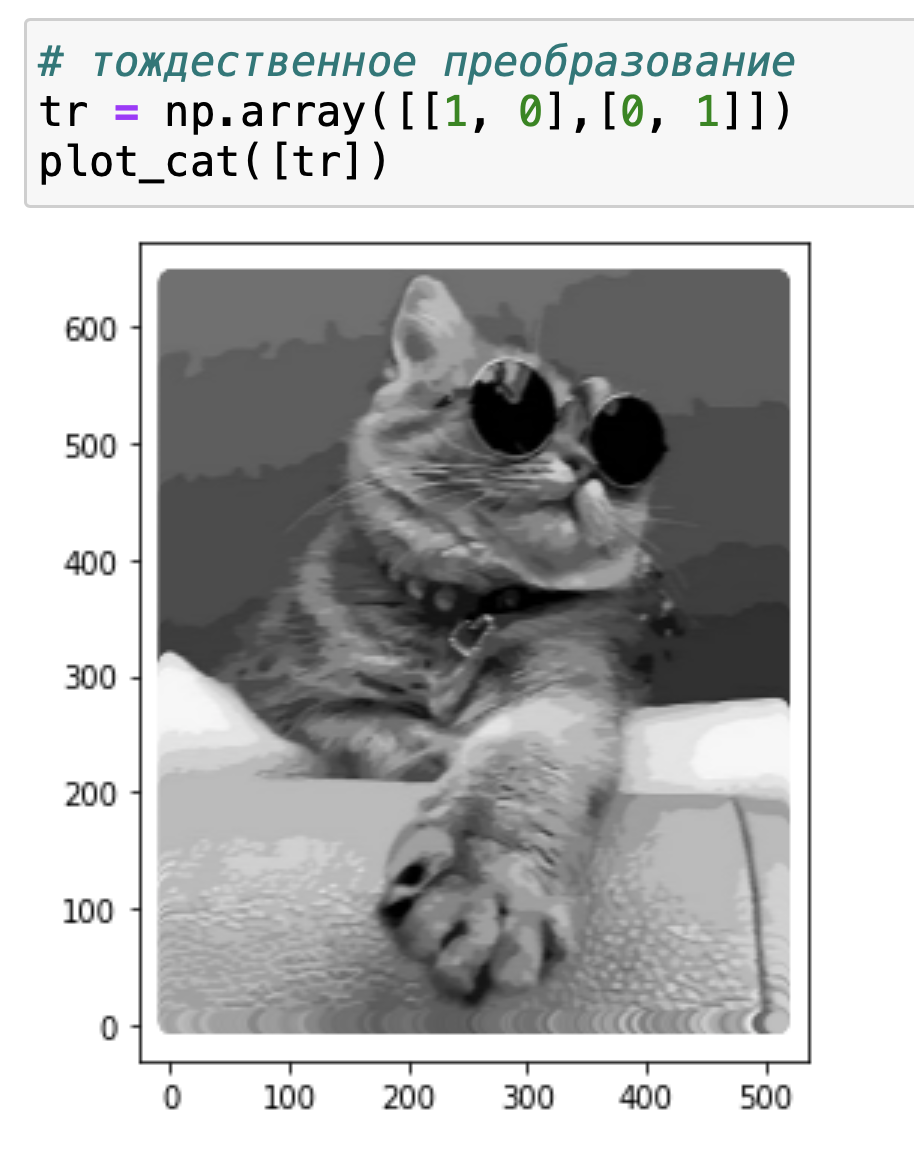
\includegraphics[scale=0.45]{id.png}
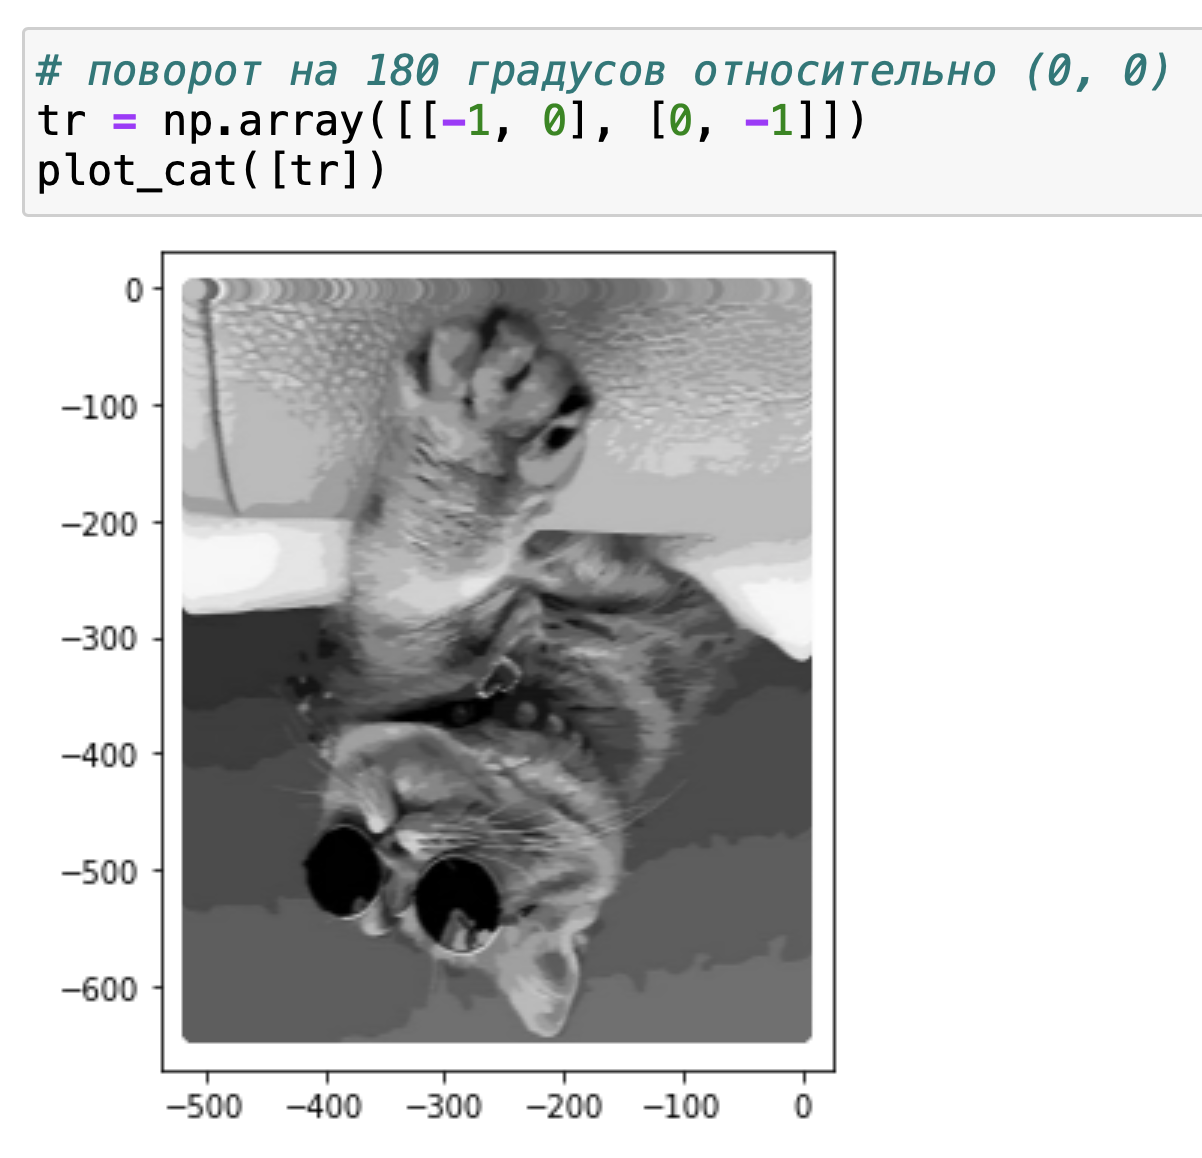
\includegraphics[scale=0.45]{rotation.png}

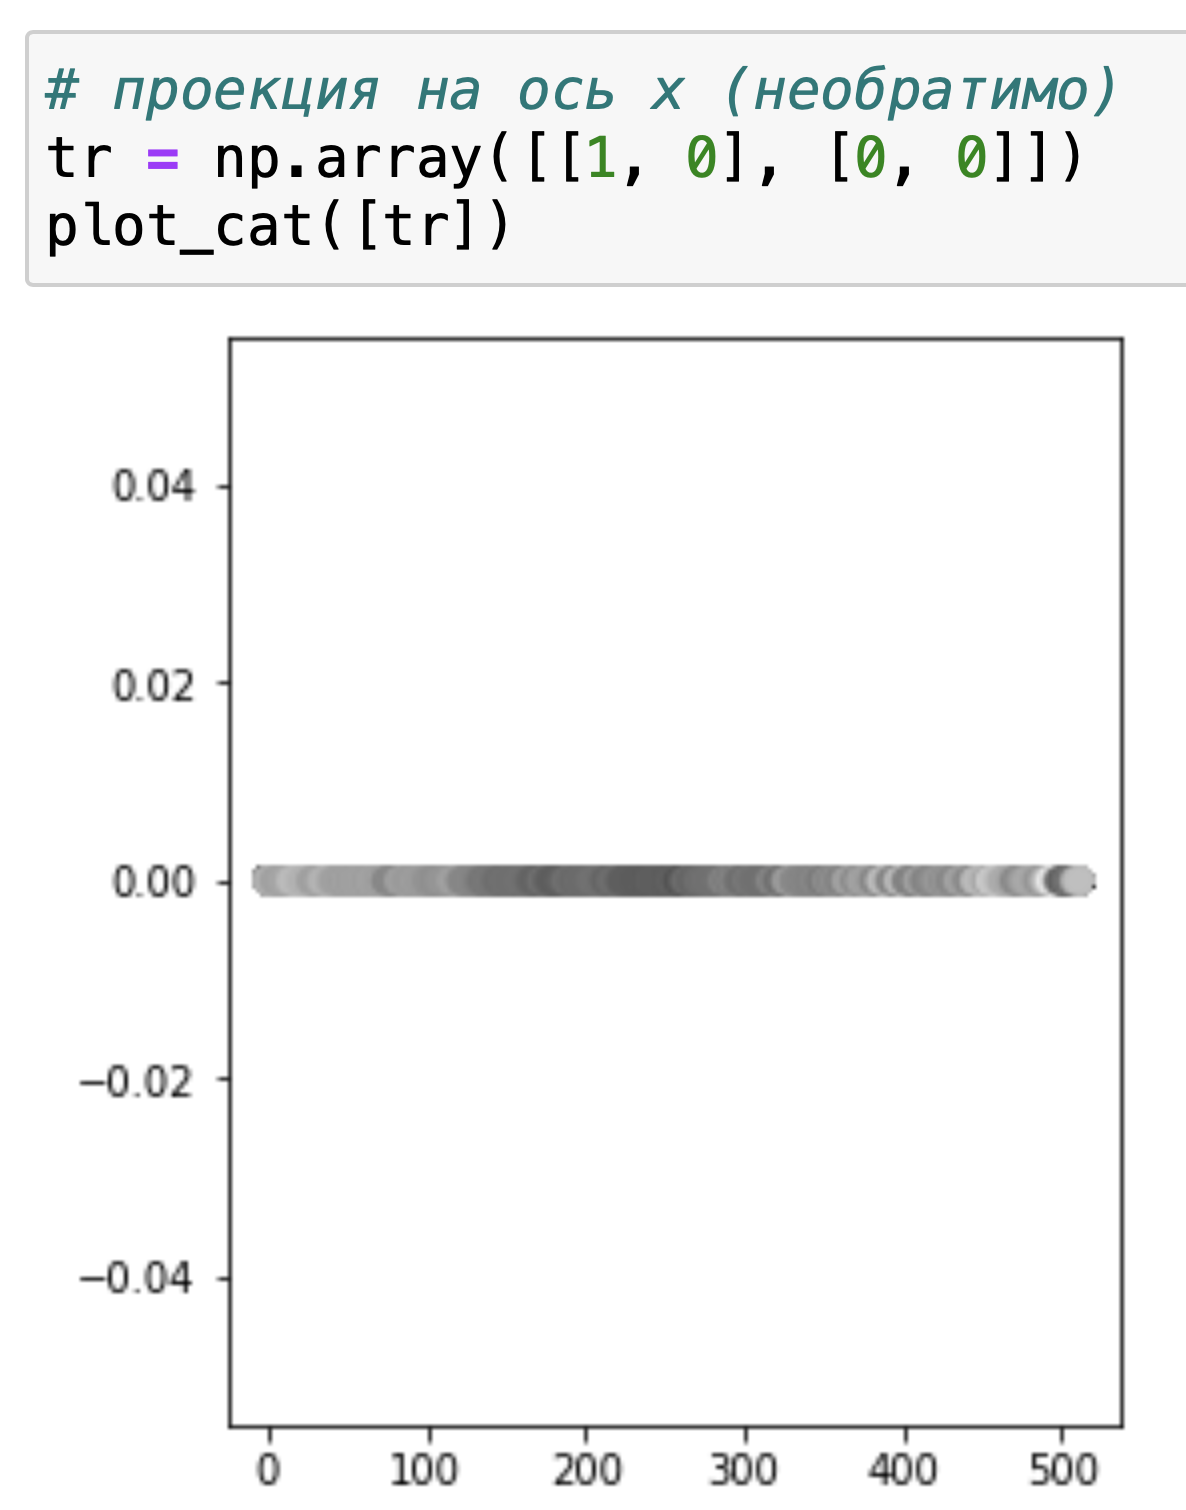
\includegraphics[scale=0.45]{projection_y=0.png}
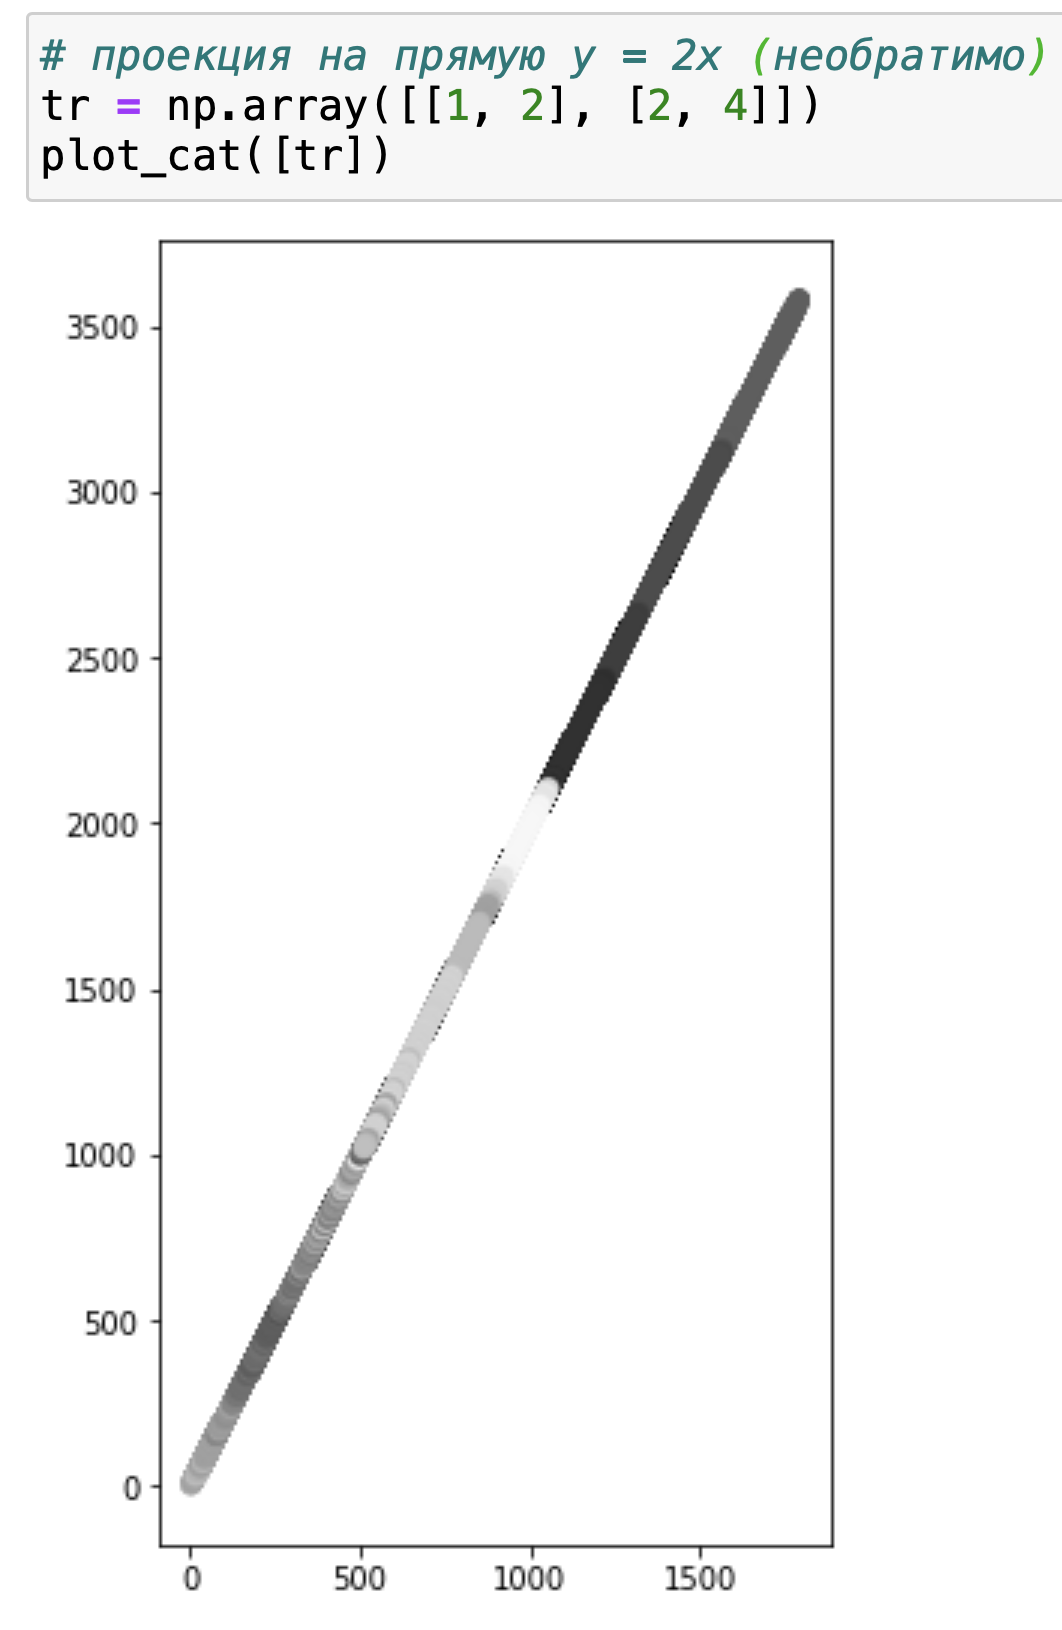
\includegraphics[scale=0.45]{projection_y=2x.png}

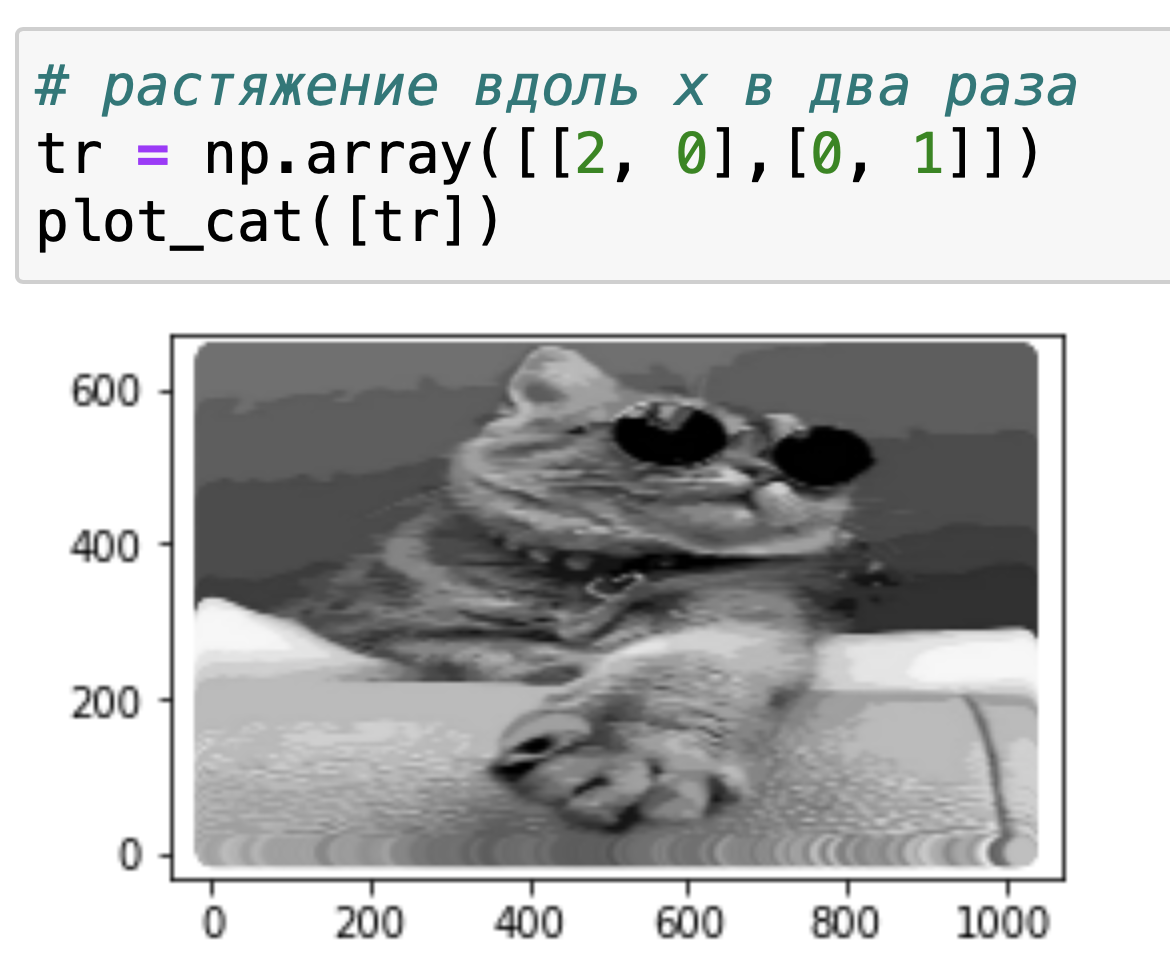
\includegraphics[scale=0.4]{streching.png}
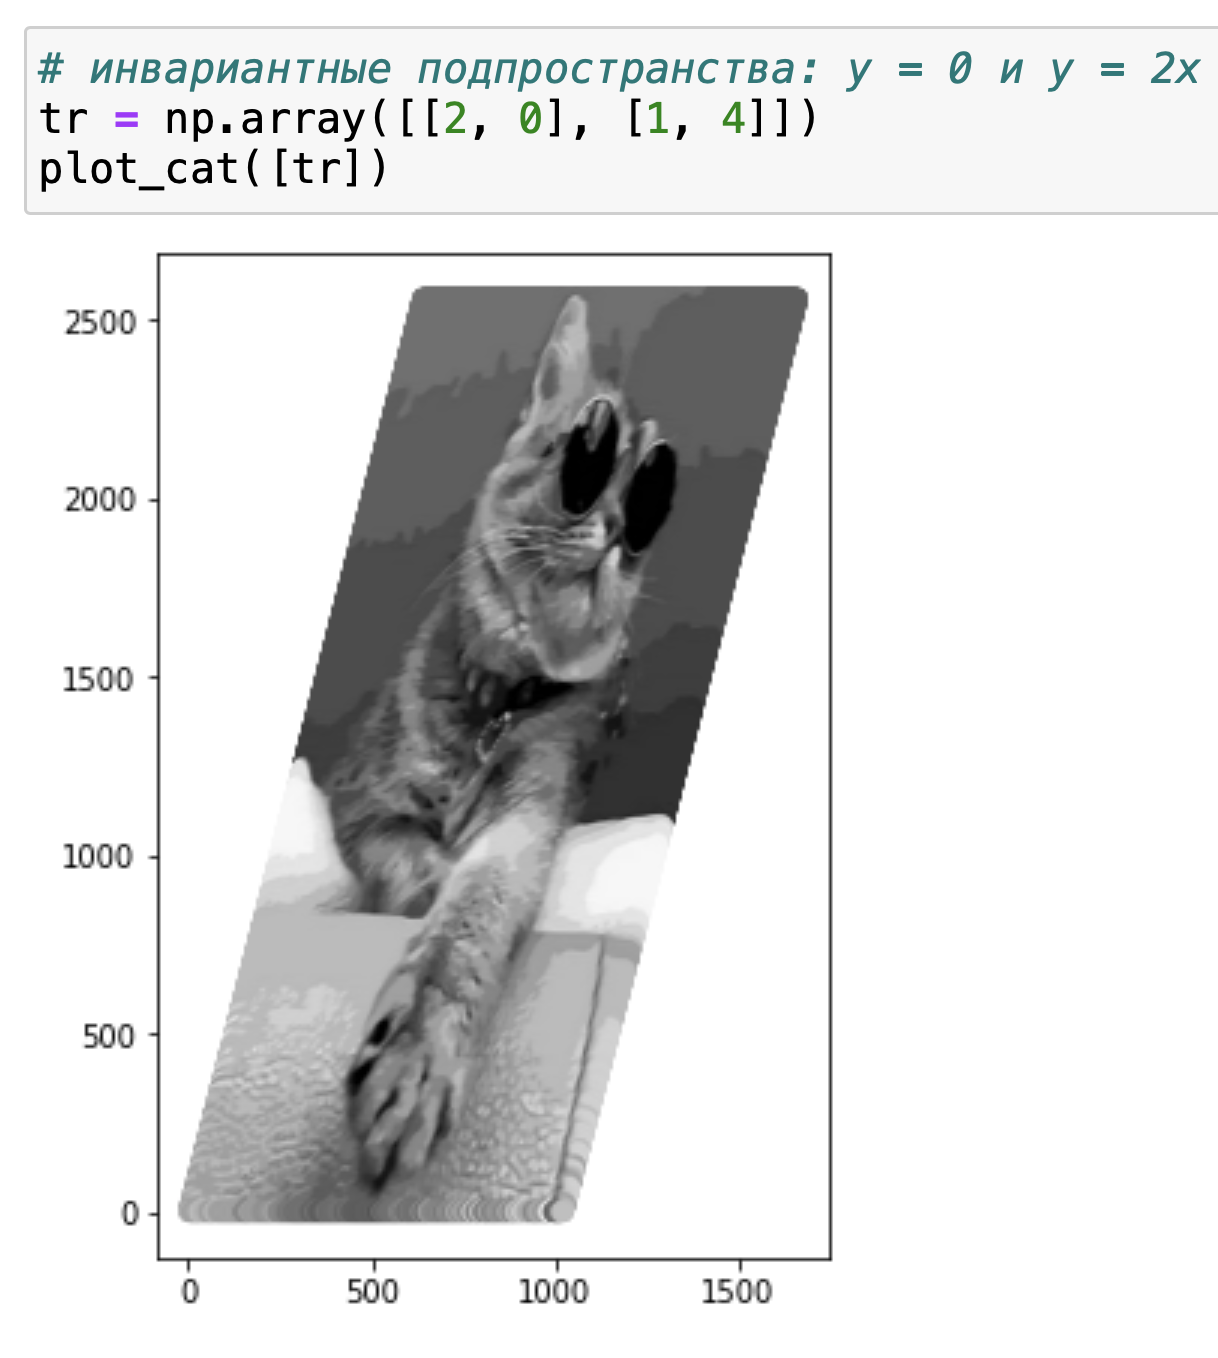
\includegraphics[scale=0.45]{invariance1.png}

\end{spacing}
\end{document}